\documentclass[11pt,compress,t,notes=noshow, aspectratio=169, xcolor=table]{beamer}

\usepackage{../../style/lmu-lecture}
% Defines macros and environments
% This file is included in slides and exercises

% Rarely used fontstyle for R packages, used only in 
% - forests/slides-forests-benchmark.tex
% - exercises/single-exercises/methods_l_1.Rnw
% - slides/cart/attic/slides_extra_trees.Rnw
\newcommand{\pkg}[1]{{\fontseries{b}\selectfont #1}}

% Spacing helpers, used often (mostly in exercises for \dlz)
\newcommand{\lz}{\vspace{0.5cm}} % vertical space (used often in slides)
\newcommand{\dlz}{\vspace{1cm}}  % double vertical space (used often in exercises, never in slides)
\newcommand{\oneliner}[1] % Oneliner for important statements, used e.g. in iml, algods
{\begin{block}{}\begin{center}\begin{Large}#1\end{Large}\end{center}\end{block}}

% Don't know if this is used or needed, remove?
% textcolor that works in mathmode
% https://tex.stackexchange.com/a/261480
% Used e.g. in forests/slides-forests-bagging.tex
% [...] \textcolor{blue}{\tfrac{1}{M}\sum^M_{m} [...]
% \makeatletter
% \renewcommand*{\@textcolor}[3]{%
%   \protect\leavevmode
%   \begingroup
%     \color#1{#2}#3%
%   \endgroup
% }
% \makeatother


\title{Interpretable Machine Learning}
% \author{LMU}
%\institute{\href{https://compstat-lmu.github.io/lecture_iml/}{compstat-lmu.github.io/lecture\_iml}}
\date{}

\begin{document}
	
	% Set style/preamble.Rnw as parent.
	
	% Load all R packages and set up knitr
	
	% This file loads R packages, configures knitr options and sets preamble.Rnw as 
	% parent file
	% IF YOU MODIFY THIS, PLZ ALSO MODIFY setup.Rmd ACCORDINGLY...
	
	% Defines macros and environments
	
	\newcommand{\titlefigure}{figure/lime5}
    \newcommand{\learninggoals}{
    	\item Learn why LIME should be used with caution}
	
	\lecturechapter{LIME Pitfalls}
	\lecture{Interpretable Machine Learning}
	
	% ------------------------------------------------------------------------------


\begin{vbframe}[allowframebreaks]{LIME Pitfalls}
  \begin{itemize}
  	\item LIME is one of the best known interpretable machine learning methods but several papers caution to be careful in their use. 
  	\item Problems can occur in several places. These are discussed in more detail below. 
  \end{itemize}
	\textbf{Pitfall: Sampling}
	\begin{itemize}
	  \item The most common sampling strategies for $\zv \in Z$ do not take the correlation between features into account. 
      \item This can lead to unlikely data points which can then be used to learn local explanation models.
      \item Ideally, we need a local sampler that samples $\zv$ from $\Xspace$. However, its derivation is particularly difficult for high dimensional or mixed feature spaces. 
      \item We could use the original training data to fit the surrogate model, but this only works well with enough data near $\xv$.
    \end{itemize}
\framebreak
	\textbf{Pitfall: Locality}
	\begin{itemize} 
     \item It is difficult to define locality (= how samples are weighted locally). It has a huge influence on the local model, but there is no automatic procedure for choosing the neighborhood.
     \item The authors of LIME proposed an exponential kernel as proximity measure between $\xv$ and $\zv$:
     	$\neigh(\zv) = exp(-d(\xv, \zv)^2/\sigma^2)$ where $d$ is a distance measure and $\sigma$ is the kernel width. 
     	 \begin{center}
     		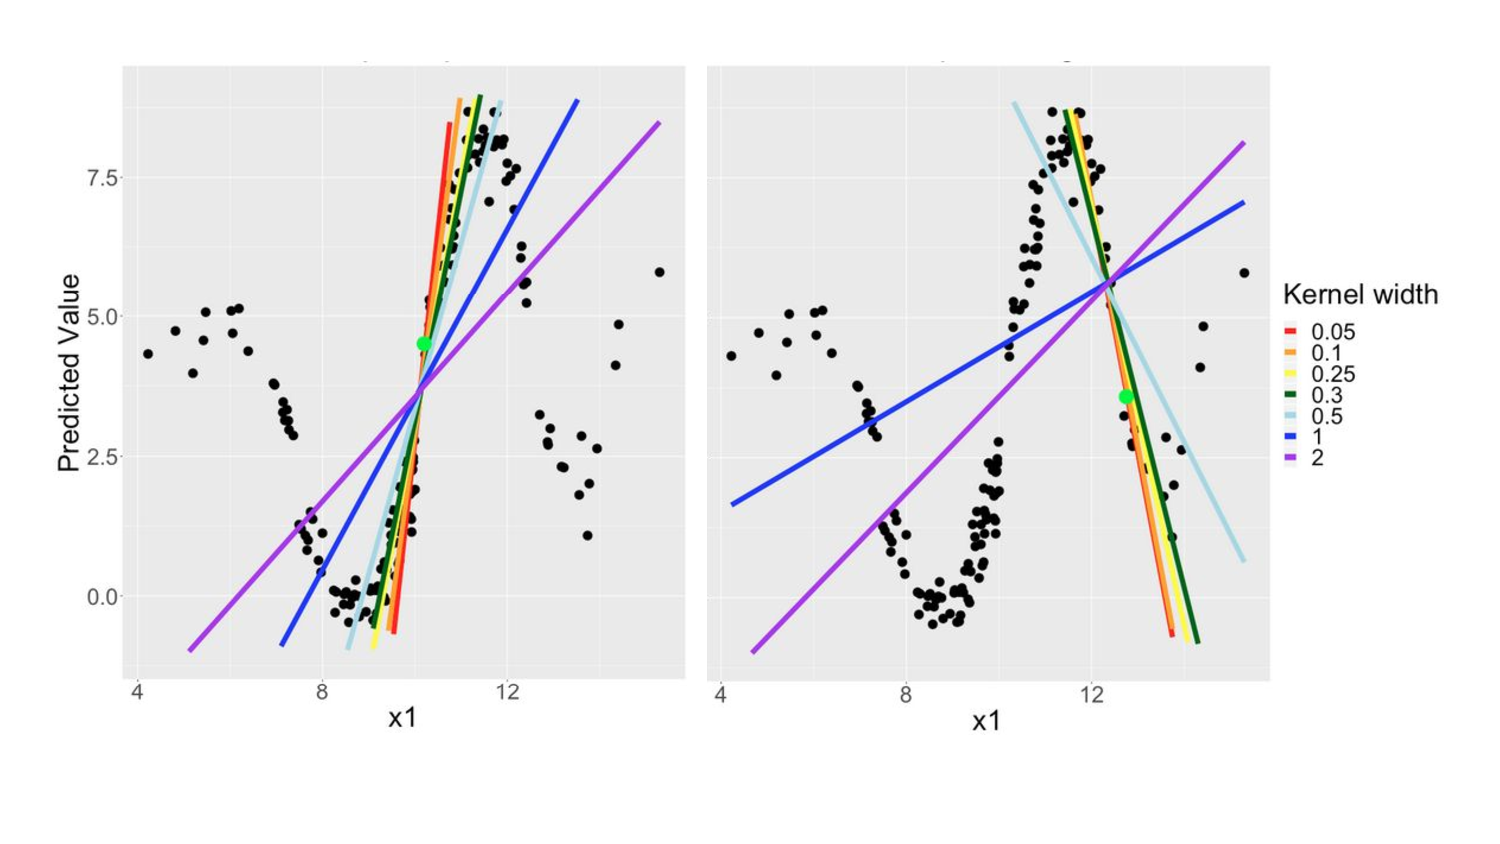
\includegraphics[width=0.6\textwidth]{figure/lime_locality}
     		\vspace{-0.5cm}
     		
     		\scriptsize{\textbf{Figure:} Linear surrogate models for two different data points based on the same model with one target and one feature. Each line displays one linear surrogate model with a different kernel width. For the data point in the right figure, larger kernel sizes are more severe.}
     		
     	\end{center}
     \item A larger kernel width means that instances that are farther away also influence the model such that we do not receive a local but a global surrogate model. 
     \item Therefore, we prefer smaller kernel widths such that an instance must be very close to influence the local model.  
     \item If the kernel width is set too small, we only fit a local model based on a few observations which carries the risk to fit noise.   
	\item Multiple software package use another default standardized distance: the Gower proximity where no kernel width needs to be specified. However, experiments showed that since also data points far away receive a weight $ > 0$, their resulting explanations are rather global surrogates than local surrogates.   
\end{itemize}
\vspace{0.3cm}

\footnote[frame]{Kopper P., Molnar M. (2019) Chapter 13 LIME and Neighborhood. In: Molnar C., Casalicchio G., König G., Pfisterer F., Scholbeck C., Bischl B. (eds) Limitations of Interpretable Machine Learning Methods. \url{https://compstat-lmu.github.io/iml_methods_limitations/}.}

\end{vbframe}

\begin{vbframe}[allowframebreaks]{LIME Pitfalls}

\textbf{Pitfall: Local vs. global features}

\begin{columns}
	\begin{column}{0.78\textwidth}
\begin{itemize}
	\item There are features that influence the \textbf{global} shape of the black-box model and \textbf{local} features that impact predictions for a small area of $\Xspace$. 
	\item For example in decision trees, splitting variables close to the root have a more global influence than the ones close to the leaves. 
	\item In most implementations, instances for the surrogate model are sampled from the whole input space which tends to hide the features with a local influence for the benefit of features with a global influence even when the kernel width was reduced. 
	\item Laugel et al. (2018) propose to sample new instances $\zv$ around the decision boundary closest from point $\xv$ for higher local accuracy.
\end{itemize}
\end{column}
\begin{column}{0.2\textwidth}

			\vspace{-0.6cm}
		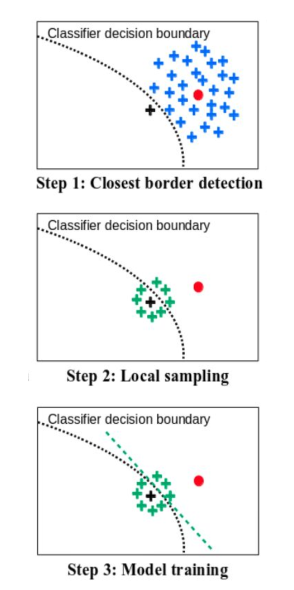
\includegraphics[width=1\textwidth]{figure/lime_bordersample2}
		
		\vspace{-0.3cm}
		
		\begin{center}
			\tiny{\textbf{Figure:} Proposed method by Laugel et al. (2018). Source: \href{http://webia.lip6.fr/~laugel/files/WHI_ICML_slides.pdf}{ICML WHI 2018}}
		\end{center}

	
 	\end{column}
\end{columns}
\framebreak
\begin{columns}
	\begin{column}{0.6\textwidth}
		\begin{itemize}
		\item Let us explain the prediction of the green dot. Background colors display predictions of a random forest, the gray line is the decision boundary.
		\item The decision boundary of LIME with default kernel width (green line) and reduced kernel width (blue line) do not match the direction of the steeper local boundary. 
		\item The method of Laugel et al. (2018) (red line) approximates the local border direction better. The red dot is the point closest to the border detected by this method. 
	\end{itemize}
\end{column}
\begin{column}{0.39\textwidth}
\vspace{0.3cm}

	\begin{center}
	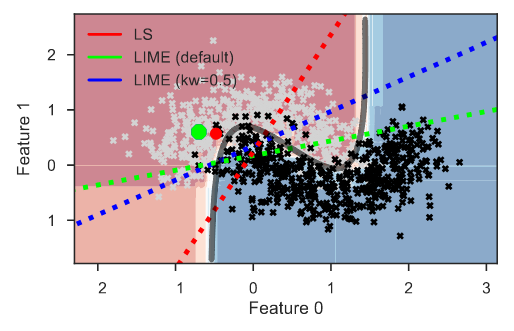
\includegraphics[width=1\textwidth]{figure/lime-globallocal2}
	
	\vspace{-0.3cm}
	{\tiny \textbf{Figure:} Half-moons dataset.}
	
\end{center}

	\end{column}
\end{columns}
\footnote[frame]{Laugel et al. (2018). Defining Locality for Surrogates in Post-hoc Interpretability. \url{https://arxiv.org/pdf/1806.07498.pdf}.}
\end{vbframe}

\begin{vbframe}[allowframebreaks]{LIME Pitfalls}
\textbf{Pitfall: Faithfulness}
\begin{itemize}
	\item There exists a trade-off between local fidelity vs. sparsity. 
	\item If the local fidelity of our interpretable model is low, we do not receive reliable explanations.
	\item On the other hand, high fidelity is only possible with a more complex model bearing the risk to substitute a black-box by a complex model that is difficult to interpret.
\end{itemize}
\framebreak

\textbf{Pitfall: Possibility to hide biases}
\begin{itemize}
	\item Slack et al. (2020) showed that data scientists could manipulate their model to hide biases. 
	\item They make use of the fact that sampled instances for the surrogate model could be out of the input data distribution if we do not account for feature dependencies. 
	\item We can built a classifier that detects whether a given data point is an out-of-distribution sample or not using the original training data and data sampled by LIME. 
	\item If a new data point has the same distribution as the training data, the prediction of the biased classifier is returned. If a new data point is out-of-distribution (usually samples for the surrogate models), the unbiased prediction is returned.
	\item For the credit dataset, a biased model could be a model solely trained on the feature `gender`, while an unbiased model could be trained on features uncorrelated with `gender` -- for example, percentage of income the credit rate represents.   
	\item Since the surrogate model is trained on out-of-distribution samples, the predictions of these samples are derived from an unbiased predictor. 
	\item Consequently, the explanations do not detect any bias although the original predictor is biased. 
\end{itemize}
\footnote[frame]{Dylan Slack et al. (2020). Fooling LIME and SHAP: Adversarial Attacks on Post hoc Explanation Methods. In Proceedings of the AAAI/ACM Conference on AI, Ethics, and Society (AIES '20). Association for Computing Machinery, New York, NY, USA, 180–186.}
\end{vbframe}

\begin{vbframe}{LIME Pitfalls}
\textbf{Pitfall: Robustness}
\begin{itemize}
	\item Another really big problem is the instability of the explanations. 
	\item Explanations of two very close points could vary greatly. 
	\item But also if $\fh$ and $\xv$ are fixed, and only new sampled data points $\zv$ are used, the resulting explanations could differ. This is called the \textbf{Rashomon Effect}.
\end{itemize}
\vspace{-0.7cm}
\begin{columns}
	\begin{column}{0.48\textwidth}
		\begin{center}
		
		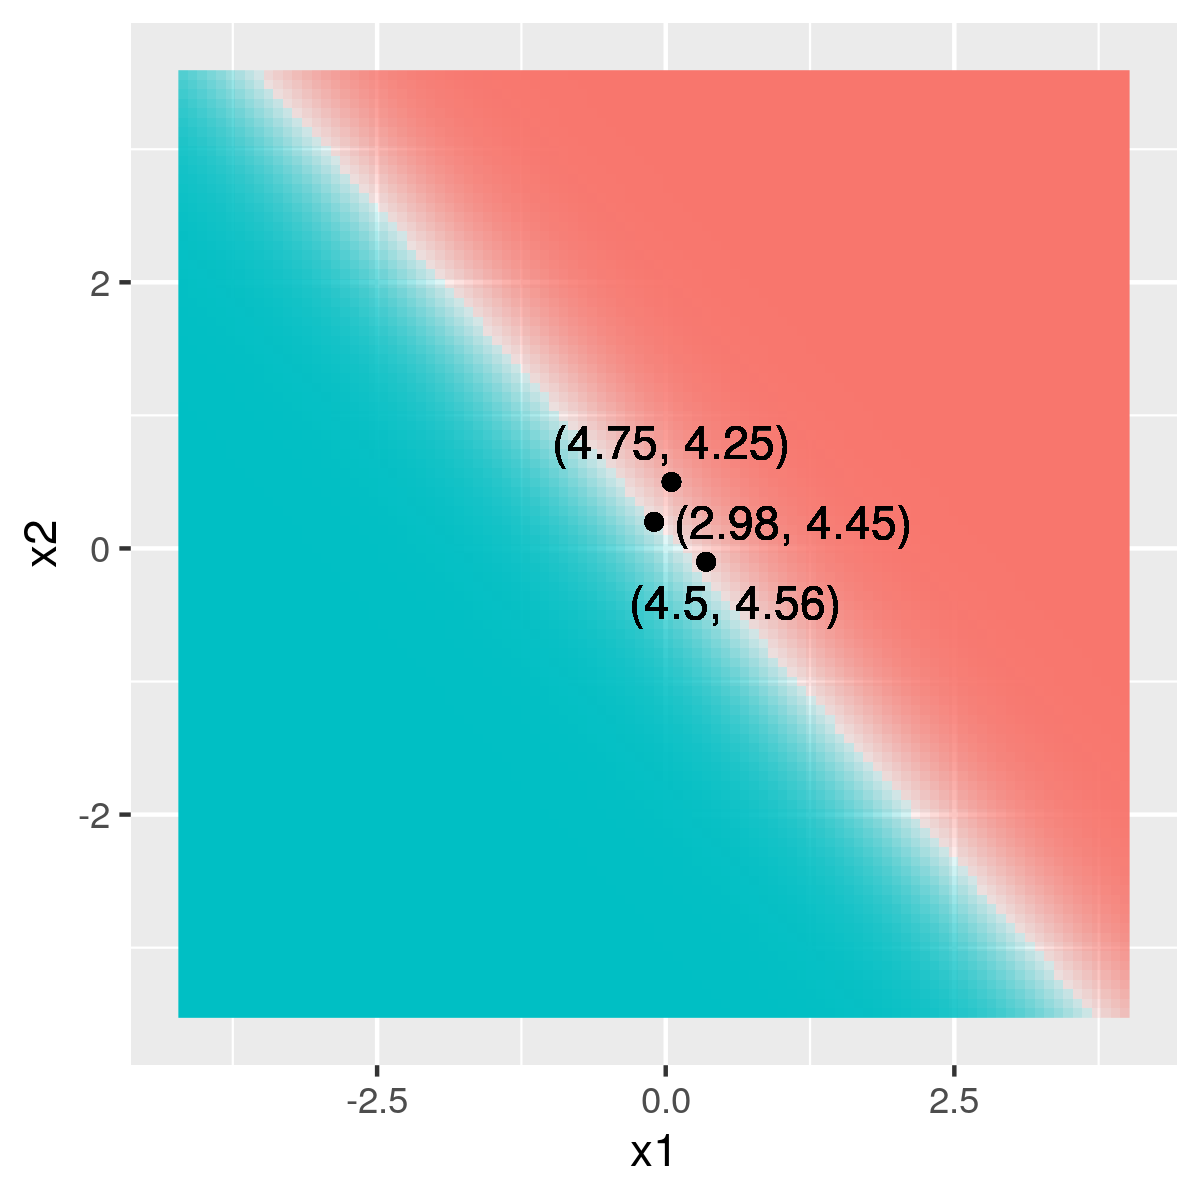
\includegraphics[width=0.55\textwidth]{figure/lime_robustness_1.png}
		
		\tiny{Figure: Linear prediction task (logistic regression). \\Linear surrogate returns similar coefficients for similar points.}
		
		\end{center}
	\end{column}
	\begin{column}{0.48\textwidth}
		\begin{center}
	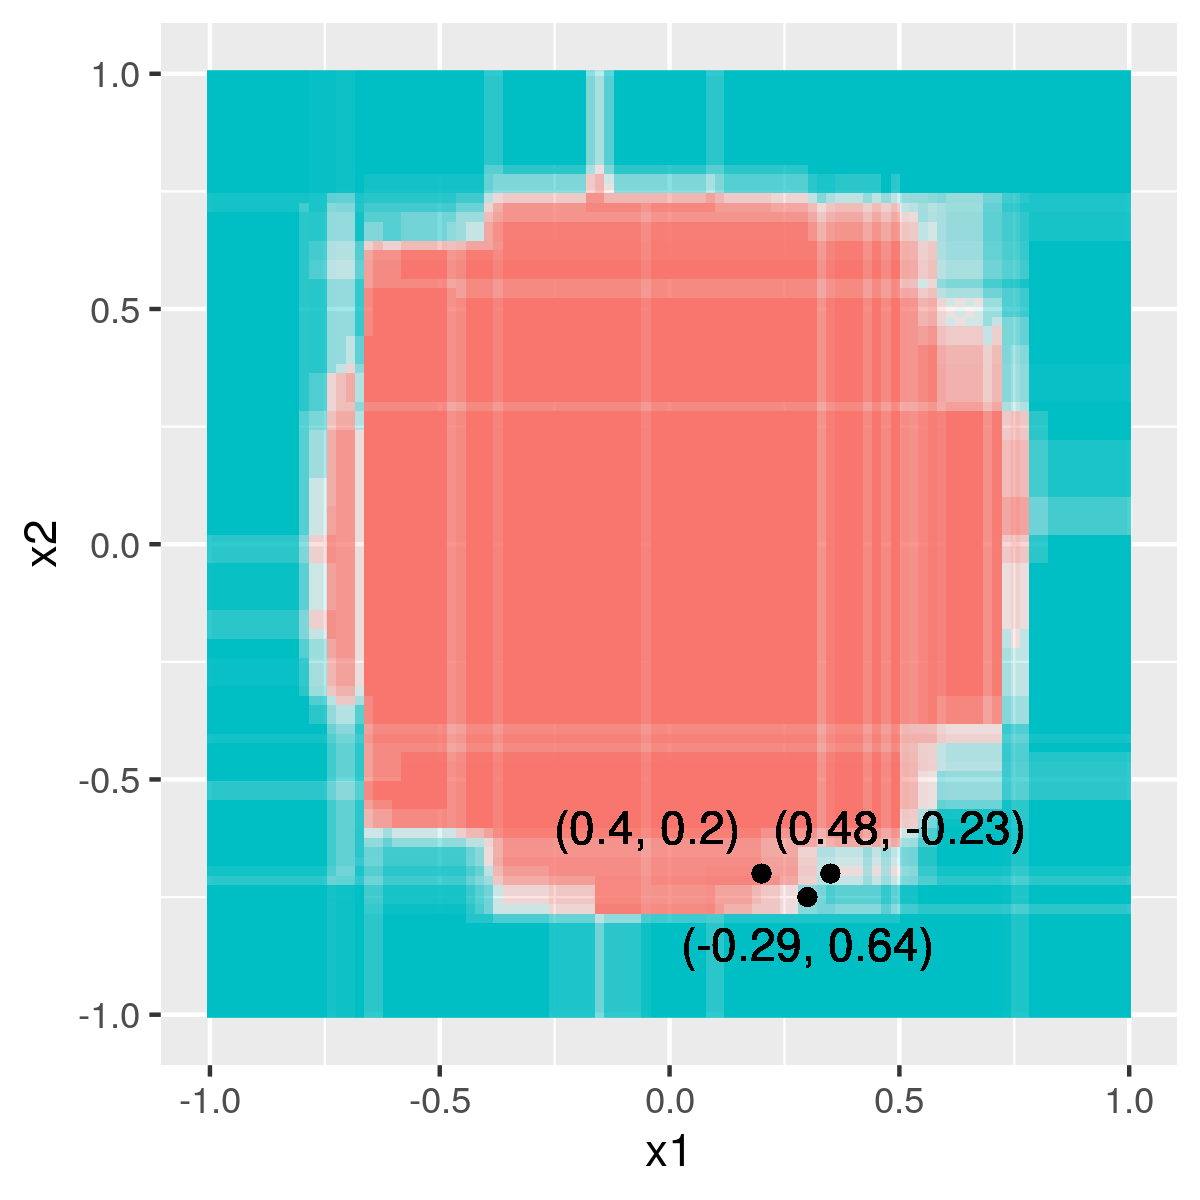
\includegraphics[width=0.55\textwidth]{figure/lime_robustness_2.png}
	
	\tiny{Figure: Circular prediction task (random forest). \\Linear surrogate returns different coefficients for similar points.}
	
	\end{center}
\end{column}
\end{columns}
\vspace{-0.2cm}
\footnote[frame]{Alvarez-Melis, D., \& Jaakkola, T. (2018). On the Robustness of Interpretability Methods. ArXiv, abs/1806.08049.}
\end{vbframe}

\begin{vbframe}{LIME Pitfalls}
\textbf{Pitfall: Definition of superpixels}
\begin{itemize}
	\item Another source of instability concerns the definition of superpixels for image data. 
	\item Multiple definitions of superpixels exist and these definitions influence both the shape and size. 
	\item The definition of superpixel has a large influence on the explanations. 
	\item Furthermore, if superpixel are only slightly changed (adversarial attack), the definitions could still differ greatly.  
\end{itemize}
\vspace{0.5cm}
\textbf{Conclusion: LIME should only be used with great caution!}

\end{vbframe}

%\begin{vbframe}{Literature}
%	\begin{itemize}
%		\small
%		\item Marco Tulio Ribeiro, Sameer Singh, and Carlos Guestrin. 2016. "Why Should I Trust You?": Explaining the Predictions of Any Classifier. In Proceedings of the 22nd ACM SIGKDD International Conference on Knowledge Discovery and Data Mining (KDD '16). Association for Computing Machinery, New York, NY, USA, 1135–1144. 
%		\item Dylan Slack, Sophie Hilgard, Emily Jia, Sameer Singh, and Himabindu Lakkaraju. 2020. Fooling LIME and SHAP: Adversarial Attacks on Post hoc Explanation Methods. In Proceedings of the AAAI/ACM Conference on AI, Ethics, and Society (AIES '20). Association for Computing Machinery, New York, NY, USA, 180–186. 
%		\item Alvarez-Melis, D., \& Jaakkola, T. (2018). On the Robustness of Interpretability Methods. ArXiv, abs/1806.08049.
%		\item Laugel et al. (2018). Defining Locality for Surrogates in Post-hoc Interpretability. \url{https://arxiv.org/pdf/1806.07498.pdf}.
%	\end{itemize}
%	
%\end{vbframe}


\endlecture
\end{document}